% Latex课程报告模板
 
\documentclass{article}
\usepackage[UTF8,zihao=-4]{ctex}

\usepackage{geometry}
\geometry{paper=a4paper}
\usepackage{graphicx}
\usepackage{gbt7714}
\usepackage{setspace}
\usepackage{indentfirst}
\usepackage{titlesec}
\usepackage{fancyhdr}    

\newCJKfontfamily\heititext{SimHei}[
  Path = C:/Windows/Fonts/,  % Windows字体目录
  AutoFakeBold = 2,        % 加粗强度(3.5为最佳视觉效果)
]


\newCJKfontfamily\simsuntext{SimSun}[
  Path = C:/Windows/Fonts/,  % Windows字体目录
  AutoFakeBold = 2,        % 加粗强度(3.5为最佳视觉效果)
]

\newCJKfontfamily\hwtext{STXinwei}[
  Path = C:/Windows/Fonts/,  % Windows字体目录
  AutoFakeBold = 2,        % 加粗强度(3.5为最佳视觉效果)
]

\begin{document}
% 自定义变量
\newcommand{\TITLE}{马克思主义自然观与科学技术观之感想} %标题
\newcommand{\AUTHOR}{周卓} %作者
\newcommand{\STUDENTNO}{2240201012} %学号

\newcommand{\sizethirty}{\fontsize{30pt}{50pt}}  % 30号字(初号)

% 行距与缩进
\onehalfspacing
\setlength{\parindent}{2em}

% 自定义各级标题格式字体
\titleformat{\section}
  {\heititext \zihao{3} \bfseries \centering}
  {\thesection}
  {1em}{}
\titlespacing{\section}{0pt}{24pt}{18pt}

\titleformat{\subsection}
  {\simsuntext \zihao{4} \bfseries \raggedright}
  {\thesubsection}
  {1em}{}
\titlespacing{\subsection}{0pt}{18pt}{12pt}

\titleformat{\subsubsection}
  {\simsuntext \zihao{-4} \bfseries \raggedright}
  {\thesubsubsection}
  {1em}{}
\titlespacing{\subsubsection}{0pt}{12pt}{6pt}

%%%%%%%%%%%%% 封面页 %%%%%%%%%%%%

\pagestyle{empty}
\begin{flushright}
{
     {\simsuntext \zihao{-4} \bfseries 2024-2025学年第二学期}
    
}
\end{flushright}


\begin{figure}[h]
    \centering
    
\includegraphics[width=0.8\textwidth]{./城院logo3.png}
    % \caption{}
\end{figure}
% \vspace*{12em}
\begin{center}
    {\hwtext\bfseries\sizethirty 
    《现代无线与移动通信系统》\\[1.5\baselineskip]  % 手动调整行距
    课程报告}
\end{center}
\begin{figure}[h]
    \centering
    
\includegraphics[width=0.33\textwidth]{./城院logo2.png}
    % \caption{}
\end{figure}
% \vspace{3em}

\newcommand{\fssi}{\fangsong\zihao{4}}

\begin{center}
{ \fssi % 这里的字号也可以用别的方式修改

\makebox[4em][s]{姓名}:\hspace{1em}\underline{\makebox[14em][c]{\AUTHOR}}\\
\vspace{1em}
\makebox[4em][s]{学号}:\hspace{1em}\underline{\makebox[14em][c]{\STUDENTNO}}\\
\vspace{1em}
\makebox[4em][s]{专业班级}:\hspace{1em}\underline{\makebox[14em][c]{电子信息2402}}\\
\vspace{1em}
\makebox[4em][s]{所在学院}:\hspace{1em}\underline{\makebox[14em][c]{信息与电气工程学院}}\\
\vspace{1em}
\makebox[4em][s]{指导老师}:\hspace{1em}\underline{\makebox[14em][c]{袁 建 涛}}\\
\vspace{1em}
\makebox[4em][s]{日期}:\hspace{1em}\underline{\makebox[14em][c]{2025.4.16}}\\
}
\end{center}



%%%%%%%%%%%%% 标题 摘要 %%%%%%%%%%%%



\title{\TITLE}
\author{\AUTHOR~ \STUDENTNO}
\date{\today}
\maketitle

\thispagestyle{empty}

\begin{abstract}
    本文首先介
    
    \textbf{关键字:} 预后模型,机器学习,智能诊断


\end{abstract}

%%%%%%%%%%%%% 目录 %%%%%%%%%%%%

\newpage
\pagestyle{plain}
\pagenumbering{roman}
\tableofcontents

%%%%%%%%%%%%% 正文 %%%%%%%%%%%%

\newpage
\pagestyle{fancy}
\fancyhf{}               % 清空默认页眉页脚
\renewcommand{\headrulewidth}{0pt} % 取消页眉线
\pagenumbering{arabic} \setcounter{page}{1} % 重置为阿拉伯数字
\cfoot{第 \thepage\ 页 \hspace{0.5em} 共 \pageref{EndBody} 页}

\section{预后模型概念}
    \subsection{基本概念}
    临床预测概率\cite{chen2020overview}.

    步骤\ref{fig:a}.
    \begin{figure}[h]
        \centering
        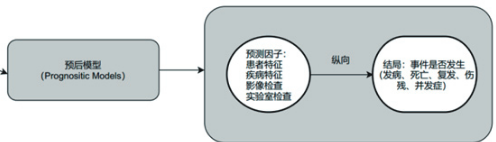
\includegraphics[width=0.5\textwidth]{2fig/a.png}
        \caption{预后模型概念}
        \label{fig:a}
    \end{figure}
    
\section{预后建模方法}
    \subsection{确立研究问题}
    
    
    \subsection{选择数据来源}

    \subsection{筛选预测变量}
   
    \subsection{处理预测变量}
    

    \subsection{拟合预测模型}
    
    \subsection{评估预测模型}
    
    
\section{机器学习在医疗领域中的应用}

    \subsection{疾病预测}
        \subsubsection{三级标题}
        高达84\%\cite{伍亚舟2022人工智能在临床领域的研究进展及前景展望}. 伍亚舟2022人工智能在临床领域的研究进展及前景展望伍亚舟2022人工智能在临床领域的研究进展及前景展望伍亚舟2022人工智能在临床领域的研究进展及前景展望伍亚舟2022人工智能在临床领域的研究进展及前景展望伍亚舟2022人工智能在临床领域的研究进展及前景展望伍亚舟2022人工智能在临床领域的研究进展及前景展望伍亚舟2022人工智能在临床领域的研究进展及前景展望伍亚舟2022人工智能在临床领域的研究进展及前景展望伍亚舟2022人工智能在临床领域的研究进展及前景展望伍亚舟2022人工智能在临床领域的研究进展及前景展望伍亚舟2022人工智能在临床领域的研究进展及前景展望伍亚舟2022人工智能在临床领域的研究进展及前景展望

    \begin{figure}[h]
        \centering
        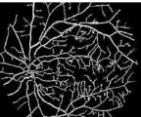
\includegraphics[width=0.5\textwidth]{2fig/b.png}
        \caption{识别血管网}
        \label{fig:b}
    \end{figure}
        
    \subsection{疾病辅助诊断}
    

\section{预后建模的挑战}
    \subsection{数据很难收集}

    \subsection{$x$数据不完备,即数据删失}

    \subsection{$\hat{y} $信息不完备,$\hat{y} $多事件且有互斥}

    \subsection{深度预后模型的可解释性}

    \subsection{数据分布偏差, 专家知识如何介入}

    \label{EndBody}        


%%%%%%%%%%%%%  参考文献 %%%%%%%%%%%%
\newpage
\pagestyle{empty}

\bibliographystyle{gbt7714-numerical}
\bibliography{2}



\end{document}